\section{Arduino Code}
To ensure the EESeaboat ("rover") operates reliably, the Arduino firmware has been designed to be lean and resilient. The Arduino does not render a webpage or handle interface concerns; its sole responsibility is processing movement and sensor requests via a simple HTTP server.

The system is designed with a clear separation between control logic and the user interface, where the Arduino acts as an HTTP server, listening for specific GET requests. The web interface (a JavaScript-based frontend) sends commands and displays responses.

This approach allows the user interface to operate independently of the rover hardware, resulting in a clear division of responsibilities:

\begin{figure}[h]
  \centering
  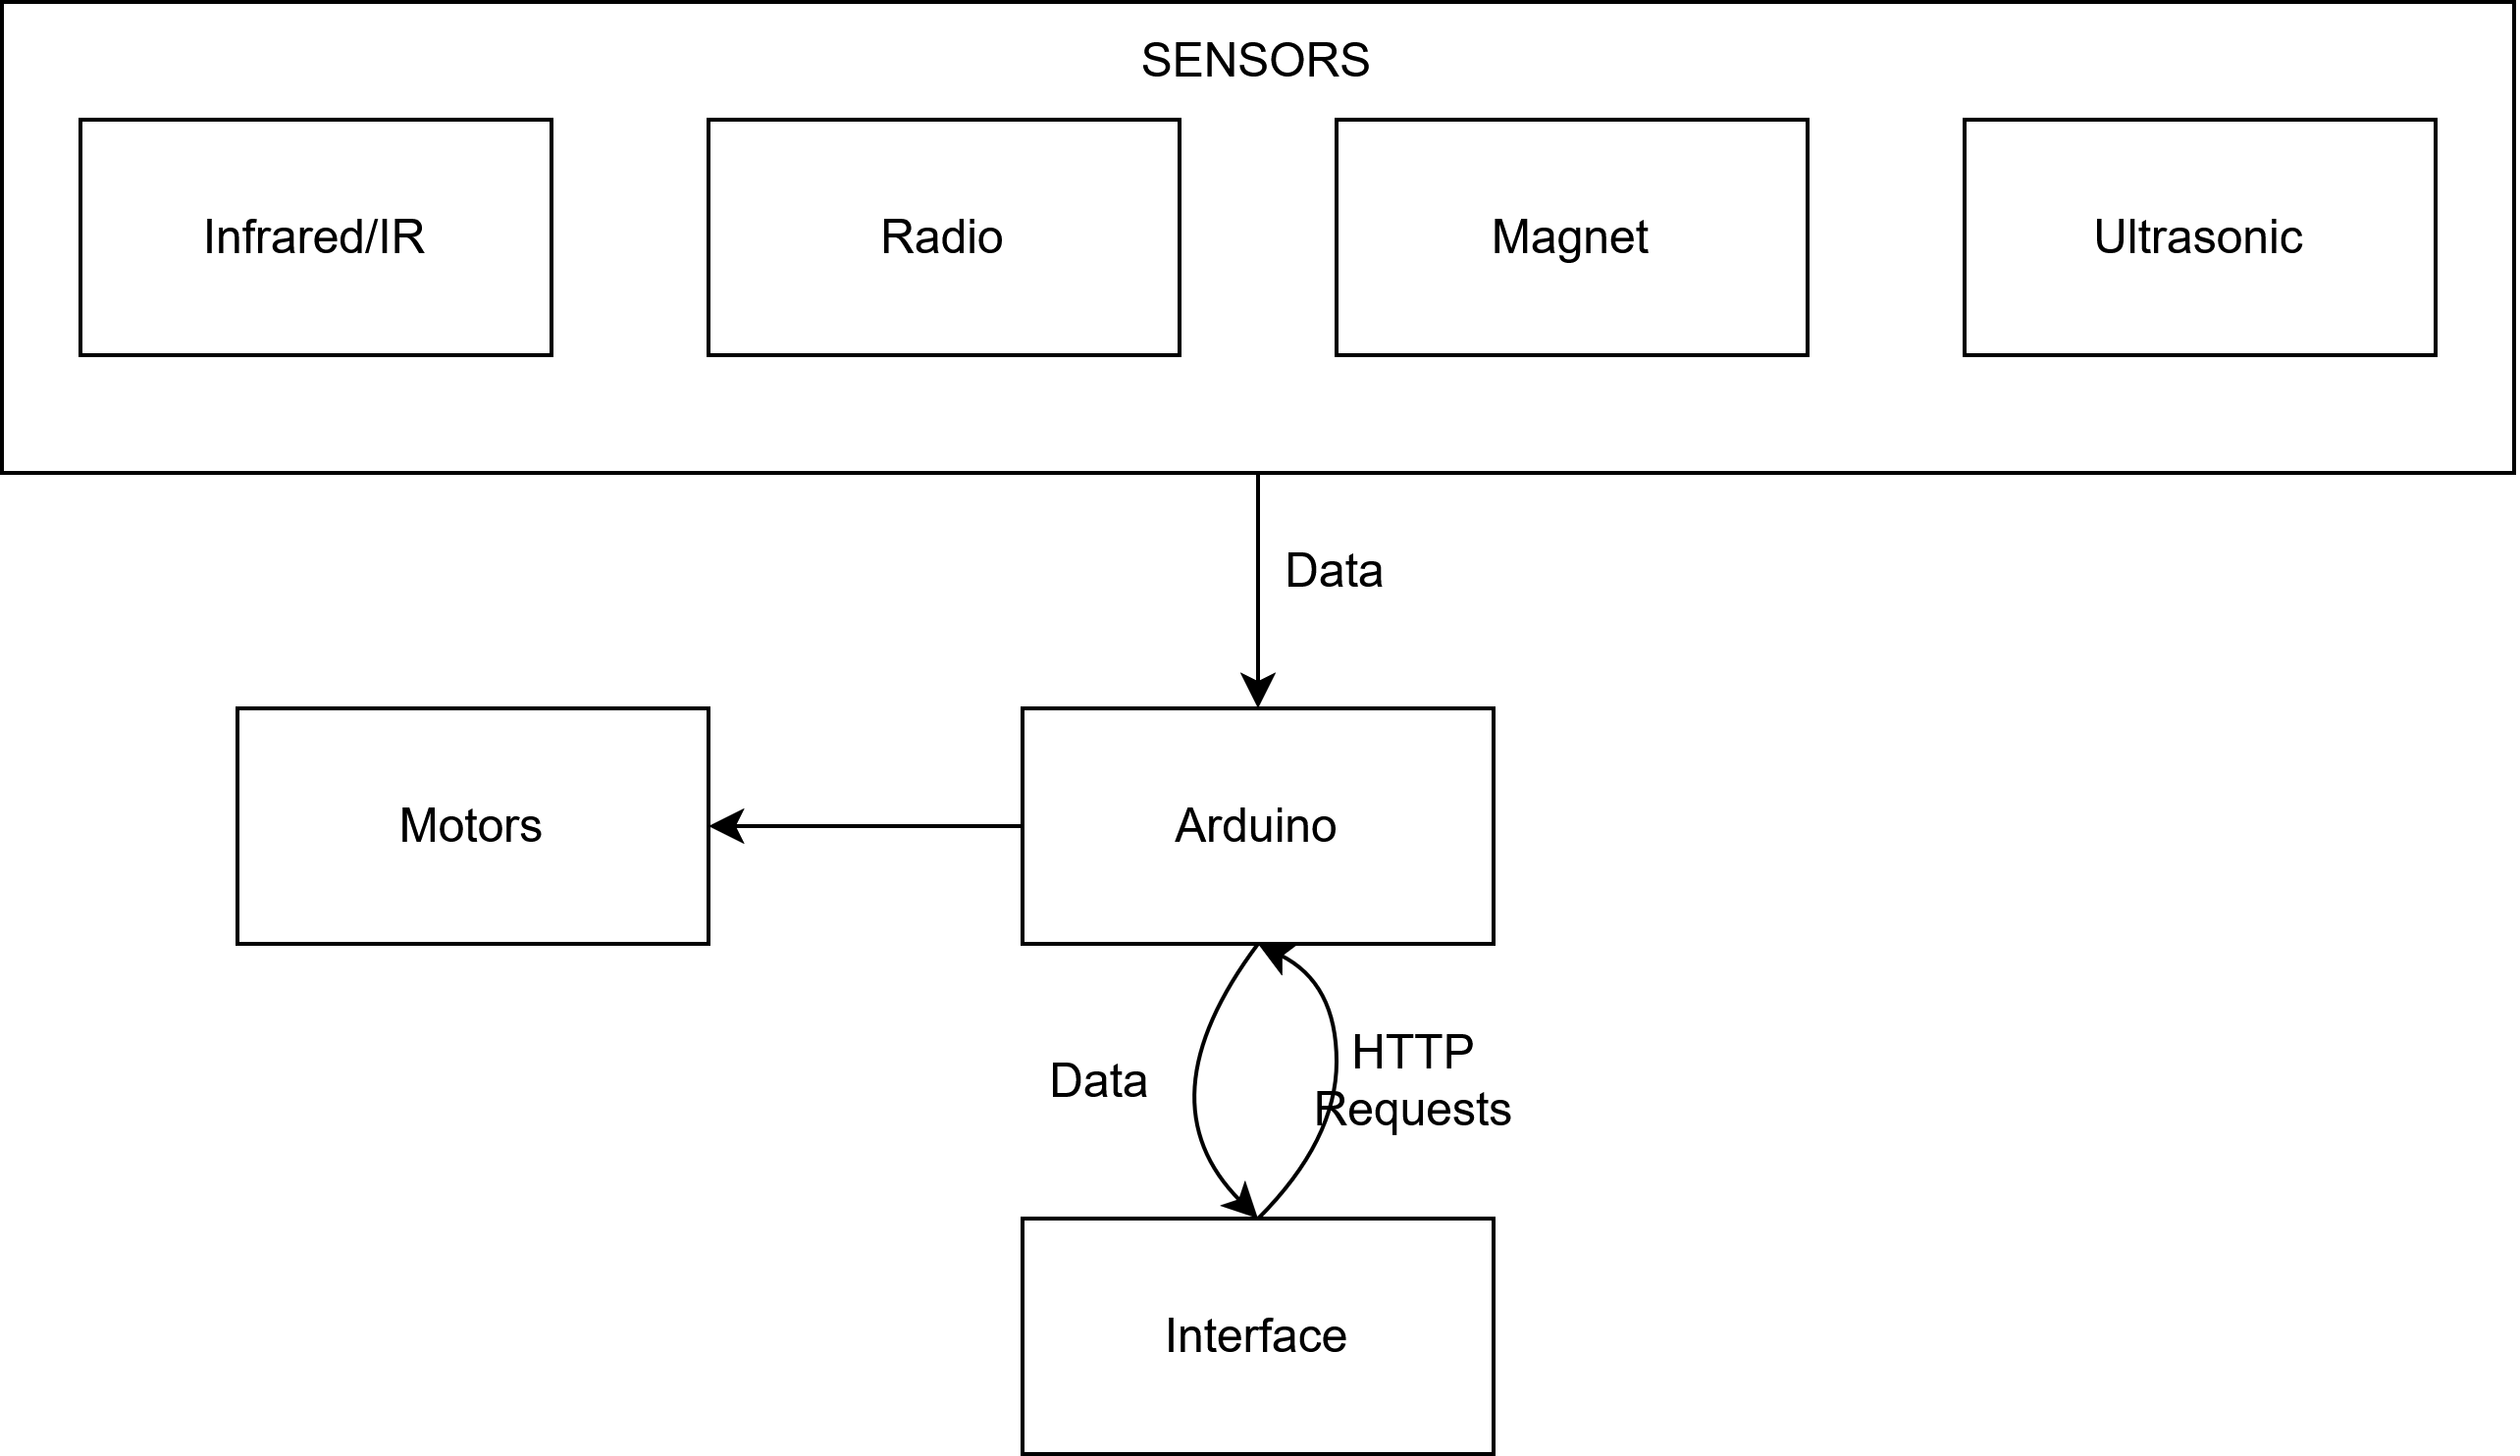
\includegraphics[width=0.8\textwidth]{subpages/images/arduino_data_flows.png}
  \caption{Data Flows Diagram}
  \label{fig:data_flows}
\end{figure}

\subsection*{Arduino as an HTTP Server}
The Arduino uses the \texttt{WiFiWebServer} library to create an HTTP server. Specific URL routes are mapped to functions using \texttt{server.on()}. Each route corresponds to a command or sensor request. A few movement examples are listed below:

\begin{verbatim}
server.on(F("/forward"), moveForward);
server.on(F("/back"), moveBack);
server.on(F("/left"), moveLeft);
server.on(F("/right"), moveRight);
server.on(F("/stop"), moveStop);
\end{verbatim}

Similar routes exist to request data from the sensors. Each function follows the same overall structure, inspired by subroutines which have a general header, body, and general exit:
\begin{itemize}
  \item Logs the received command to the Serial Monitor for debugging.
  \item Executes the main body of the specific function.
  \item Responds with an HTTP status and text message.
\end{itemize}

As an example, moving left is defined as below:

\begin{verbatim}
void moveLeft()
{
  Serial.println(F("[INFO] Command: Move Left"));
  digitalWrite(leftMotorPin, LOW);
  digitalWrite(rightMotorPin, HIGH);
  digitalWrite(leftMotorDirPin, HIGH);
  digitalWrite(rightMotorDirPin, HIGH);

  server.sendHeader("Access-Control-Allow-Origin", "*");
  server.send(200, F("text/plain"), F("Moving Left"));
}
\end{verbatim}

This pattern ensures each route is stateless and compatible with asynchronous HTTP communication.

Additional routes were defined to handle sensor readings. These include:
\begin{itemize}
  \item \texttt{/IR} - Returns the frequency of the infrared sensor.
  \item \texttt{/radio} - Returns the frequency of the radio signal.
  \item \texttt{/magnet} - Returns the magnetic direction (NORTH/SOUTH).
  \item \texttt{/ultra} - Returns a duck’s name embedded in the ultrasonic data.
\end{itemize}

Each handler processes the sensor reading and sends back a text response in a consistent, parseable format (e.g., \texttt{"457Hz"} or \texttt{"Name: Wibbo"}).

\subsection*{Web Interface}
\begin{figure}[h]
  \centering
  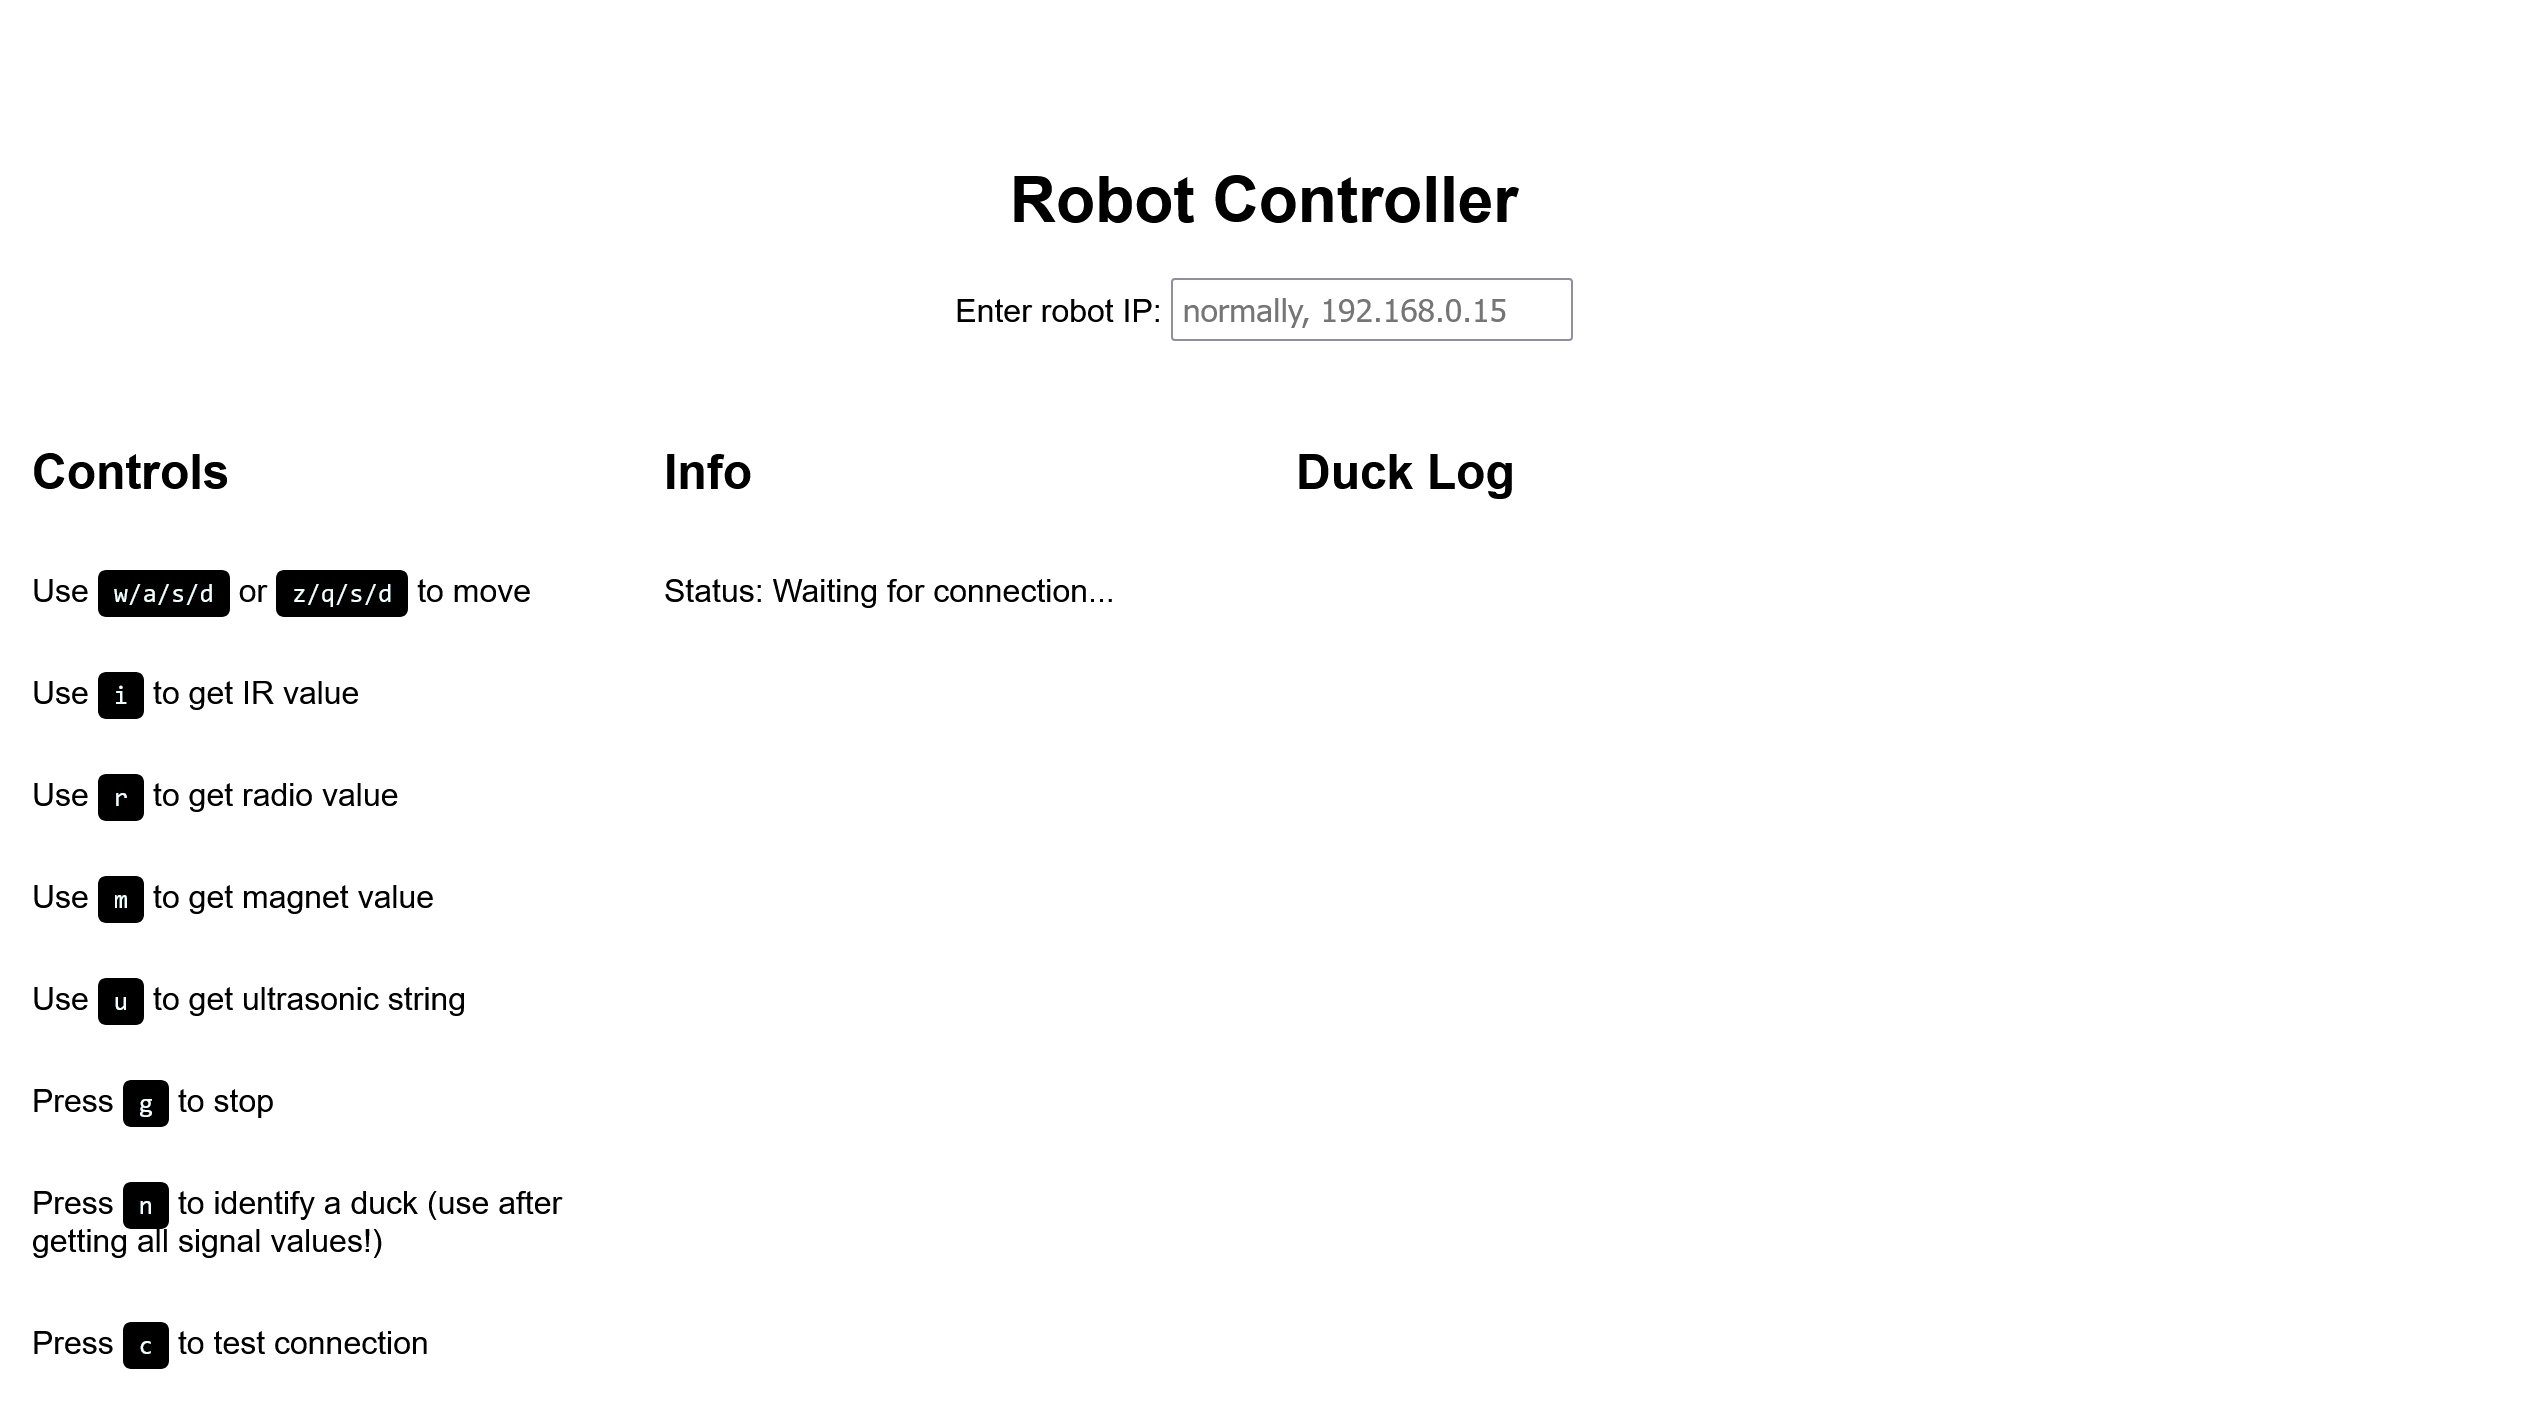
\includegraphics[width=0.8\textwidth]{subpages/images/early_web_interface.png}
  \caption{Early Version of User Interface}
  \label{fig:early_web_interface}
\end{figure}

The front-end is a JavaScript-based web application. It uses keyboard input to send commands to the rover over HTTP, using the \texttt{fetch()} API. The user specifies the rover’s IP address, then interacts using intuitive keybindings (\texttt{wasd} for movement and initials for other). The script tracks active keys and suppresses duplicate requests, especially for movement commands, to minimize redundant traffic.

\begin{verbatim}
fetch(`http://${ip}/${command}`)  
      .then(res => res.text())  
      .then(text => {  
          statusDisplay.textContent = text;  
   // ... more here ...  
      })  
      .catch(err => {  
          console.error(err);  
          statusDisplay.textContent = "Failed to connect";  
      });
\end{verbatim}

This function is responsible for funneling user interaction to send the correct request to the Arduino.

\subsection*{Duck Identification}
To classify ducks, each has a species-specific sensor signature comprising:
\begin{itemize}
  \item Infrared frequency
  \item Radio frequency
  \item Magnetic orientation
\end{itemize}

The identification logic maps these attributes to known species using tolerance-based matching. The logic table from the project brief is encoded as follows:

\begin{center}
  \begin{tabular}{|c|c|c|c|}
    \hline
    Species & Infrared & Radio & Magnetic \\
    \hline
    Wibbo   & 457Hz    &       & Down     \\
    Gribbit &          & 100Hz & Down     \\
    Snorkle & 293Hz    &       & Up       \\
    Zapple  &          & 150Hz & Up       \\
    \hline
  \end{tabular}
\end{center}

We keep these variables in the code:
\begin{verbatim}
let magnetDir = "";
let irFreq = 0;
let radioFreq = 0;
let duckName = "";
\end{verbatim}

Upon pressing the \texttt{n} key, the function \texttt{newDuck()} checks against the table:
\begin{verbatim}
const TOLERANCE = 10;
if (Math.abs(irFreq - 457) <= TOLERANCE && magnetDir === "SOUTH") {
  species = "Wibbo";
} else if (Math.abs(radioFreq - 100) <= TOLERANCE && magnetDir === "SOUTH") {
  species = "Gribbit";
} else if (Math.abs(irFreq - 293) <= TOLERANCE && magnetDir === "NORTH") {
  species = "Snorkle";
} else if (Math.abs(radioFreq - 150) <= TOLERANCE && magnetDir === "NORTH") {
  species = "Zapple";
}
\end{verbatim}

The species name and duck name are then timestamped and inserted into the “Duck Log” section of the UI. If no match is found, the user is prompted to verify that all sensor readings have been collected.

\subsection*{Sensor Processing}
Each sensor on the rover provides a signal for duck classification and is accessed via a dedicated HTTP route. The Arduino reads the sensor data, processes it as needed, and returns a plain-text response that the browser can easily interpret. Not shown here is code for error handling, which is done by sending an HTTP status 400 and an error string to the interface if there is no output from sensors, or if the output doesn’t match expected outcomes.

\subsubsection*{Infrared and Radio Frequency Sensors}
Both the infrared and radio sensors are connected to analog input pins. The Arduino measures their signal frequency using the \texttt{pulseIn()} function and computes the corresponding Hertz value, by measuring the high and low time to get the period. A simplified version of the functionality is shown below:

\begin{verbatim}
float getFreq(int pin) {
  unsigned long highTime = pulseIn(pin, HIGH, 50000);
  unsigned long lowTime = pulseIn(pin, LOW, 50000);
  if (highTime == 0 || lowTime == 0) return 0;
  return 1000000.0 / float(highTime + lowTime);
}
\end{verbatim}

This then gets sent to the interface through each respective route, a frequency string like \texttt{"457.00Hz"} that the JavaScript interface extracts and compares to known species ranges.

\subsubsection*{Magnetic Sensor}
The rover uses a Hall effect sensor to detect the magnetic's field polarity. The Arduino reads an analog voltage that varies depending on the pole facing the sensor.

\begin{verbatim}
int rawValue = analogRead(magnetPin);
float voltage = rawValue * (3.3 / 1023.0);
\end{verbatim}

The sensor outputs roughly 2.5V with no field, >2.05V for South polarity (DOWN), and <1.98V for North polarity (UP). Based on this, the Arduino classifies the magnetic direction:

\begin{verbatim}
if (voltage >= 2.05) {
  server.send(200, "text/plain", "SOUTH");
} else if (voltage <= 1.98) {
  server.send(200, "text/plain", "NORTH");
} else {
  server.send(400, "text/plain", "ERROR: Invalid magnet reading");
}
\end{verbatim}

This method is more precise than using a binary input and allows detection even with weak magnetic fields. The output is returned as \texttt{"NORTH"} or \texttt{"SOUTH"} for frontend classification logic.

\subsubsection*{Ultrasonic Sensor}
The ultrasonic system transmits a 4-character string over a slow UART serial link (e.g., \#Eve). The Arduino waits for the start character, ‘\#’ and then reads the remaining three letters as the name. It uses \texttt{Serial1} to read the signal at a baud rate of 600 to match the bit rate of the signal.

The process is robust against garbage data and timeouts:

\begin{verbatim}
while (!foundStart && (millis() - startTime < 1000)) {
  if (Serial1.available()) {
    charIn = Serial1.read();
    if (charIn == '#') {
      name += charIn;
      foundStart = true;
    }
  }
}
\end{verbatim}

After receiving the start marker, the remaining characters are read one at a time with small delays to accommodate the slow baud rate:

\begin{verbatim}
while (name.length() < 4) {
  if (Serial1.available()) {
    charIn = Serial1.read();
    name += charIn;
  }
}
\end{verbatim}

The name then gets returned to the interface to continue the duck identification.

\subsection*{Movement}
Using the given H-Bridge Motor Driver Module, we can connect the corresponding pins for each motor’s movement and direction to inputs to the Arduino. Then, depending on the movement command received, the motors are driven at appropriate speeds and directions using the following function:

\begin{verbatim}
void setMotorSpeed(int leftSpeed, int rightSpeed, bool leftForward, 
bool rightForward)
{
  analogWrite(leftMotorPin, leftSpeed);
  analogWrite(rightMotorPin, rightSpeed);
  digitalWrite(leftMotorDirPin, leftForward ? HIGH : LOW);
  digitalWrite(rightMotorDirPin, rightForward ? HIGH : LOW);
}
\end{verbatim}

Using \texttt{analogWrite} for the speed, we can drive motors at different voltages to allow for diagonal movement.

\section{CAD}
To keep things simple with the design, we used the given chassis, which allowed us to spend more time working on the more pressing issues. However, we knew that space would be tight if we didn’t add anything to the original chassis. We wanted to push the chassis to the extreme, so we looked at what was available to be worked with. The chassis has two holes at the front, originally meant for servo motors. We decided to repurpose these to place a mount, which would hold our ill-fitting circuitry and all the sensors. A thing to keep in mind here was the weight, as the original chassis is already close to half the permitted weight, something kept in mind throughout the project.

In total four parts where designed and added to the chassis to allow for proper operation of the rover.

\subsection*{Breadboard Box and Infrared Sensor Shield}
\begin{figure}[H]
  \centering
  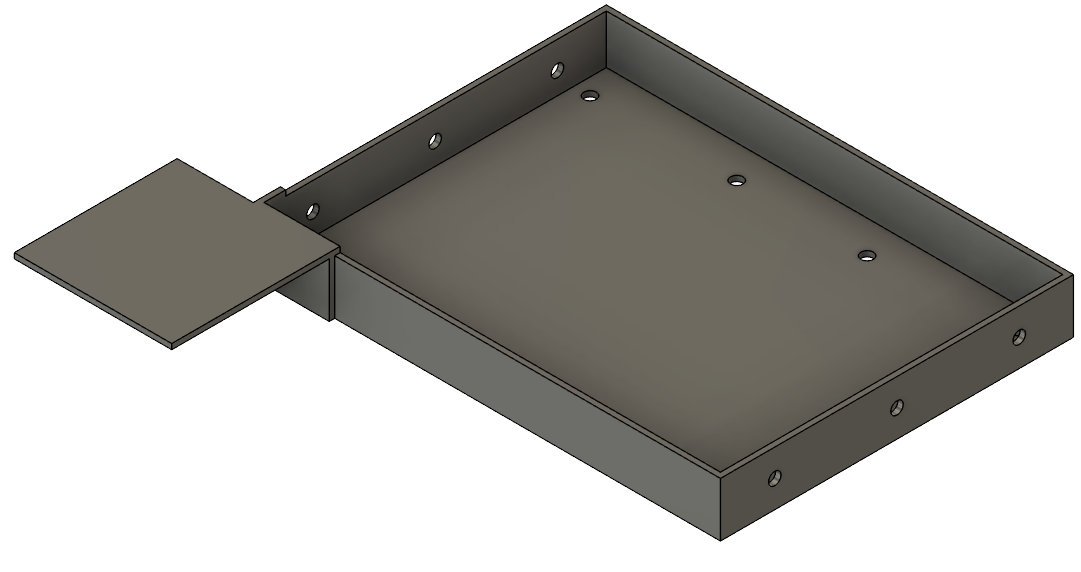
\includegraphics[width=0.7\textwidth]{subpages/images/breadboard_box.png}
  \caption{Mount for Breadboard with a Shield for Phototransistor}
  \label{fig:breadboard_box_shield}
\end{figure}
This enclosure accommodates a breadboard for additional circuit components, enabling larger and cleaner circuit layouts by providing extra space for separation and organization. The box includes a dedicated side mounting points for the infrared and other sensor, and features a cover designed to shield the infrared sensor from ambient light interference, thereby improving measurement accuracy.

\subsection*{Magnetic Sensor Arm Mount}
\begin{figure}[H]
  \centering
  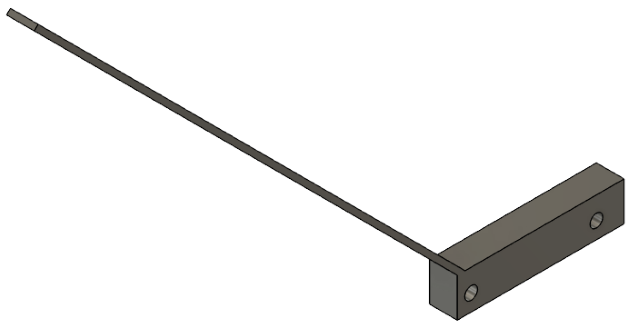
\includegraphics[width=0.7\textwidth]{subpages/images/magnet_arm.png}
  \caption{Arm Mount for the Hall Sensor}
  \label{fig:magnet_arm}
\end{figure}
To optimize detection, the magnetic sensor must be positioned above the duck’s head. A vertical arm was designed to elevate the sensor to the correct height while anchoring it to the box, ensuring consistent alignment during operation.

\subsection*{Ultrasonic Sensor Housing}
\begin{figure}[H]
  \centering
  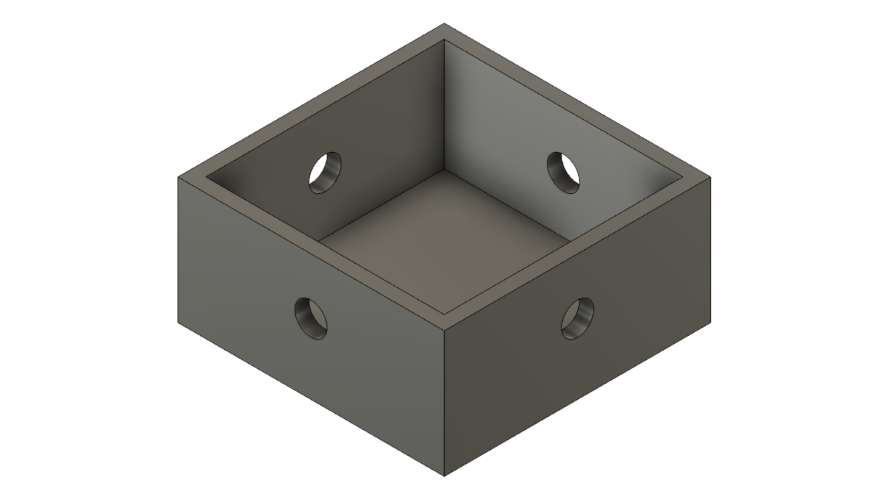
\includegraphics[width=0.7\textwidth]{subpages/images/ultrasonic_mount.png}
  \caption{Holder for the Ultrasonic Sensor}
  \label{fig:ultrasonic_mount}
\end{figure}
Due to form factor limitations, the ultrasonic sensor could not be mounted directly to the chassis. A dedicated enclosure was designed with pass-through holes for wiring, providing a secure mounting location and easy access to the sensor for UART signal processing.